\subsection{Loss-of-function variants in HG002}
Of the \NVariants{} variants, \NCoding{} have a coding or canonical
splice-site consequence in a MANE Select transcript and \NPlof{} a pLoF
consequence. The filters retain \NHc{} high-confidence pLoF variants in
\NHcGenes{} genes (Figure~\ref{fig:funnel}); \NHcRare{} are rare,
\NHcCommon{} have a frequency of at least 1\%, and \NHcHom{} are homozygous.
Each tier removes a different kind of false or uninformative LoF call
(Table~\ref{tab:lofflags}). The frequency filter of tier~1 removes pairs of
nearby frameshifts at a frequency of 100\% that together restore the
reading frame, in \textit{SON} (+1 and $-$1\,nt) and \textit{SLAIN1} (+2 and
+1\,nt), i.e.\ positions at which GRCh38 carries a rare sequence, and the
\textit{FMO2} p.Gln472Ter allele (\textit{FMO2*2}, 99.5\%), which inactivates
\textit{FMO2} in most humans. ClinVar removes, among others, the
\textit{LPL} p.Ser474Ter allele (S447X in the legacy numbering), a
stop-gain that is classified benign, and the \textit{CYP2D6*4} splice-acceptor
variant, which is classified as a drug-response allele; the latter also lies
in a segmental duplication, as do pLoF calls in olfactory receptor,
\textit{NBPF}, \textit{GOLGA8} and \textit{NPIPB} genes.

\begin{figure}[ht]
\centering
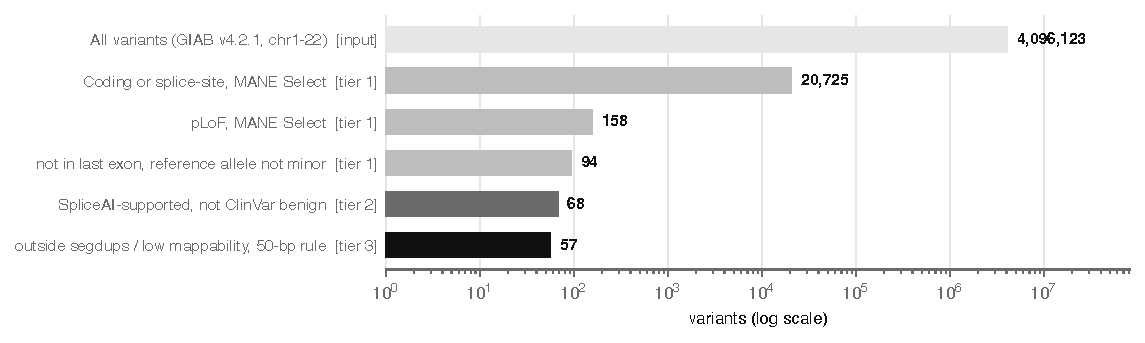
\includegraphics[width=0.85\textwidth]{figures/figS_funnel.pdf}
\caption{Variants of HG002 retained at each step. The pLoF steps count
variants with at least one MANE Select pLoF consequence that passes the
filters of the tiers applied so far (log scale; shading by tier).}
\label{fig:funnel}
\end{figure}

\begin{table}[ht]
\centering\small
\begin{tabular}{llp{0.42\textwidth}r}
\toprule
Tier & Flag & Source & Variants \\
\midrule
1 & last exon & \texttt{EXON} of the MANE Select consequence & \FlagLastExon{} \\
1 & allele frequency $\geq$ 95\% & gnomAD exomes/genomes in the core cache & \FlagRefMinor{} \\
2 & no SpliceAI support & SpliceAI plugin, all delta scores $<$ 0.2 & \FlagSpliceai{} \\
2 & ClinVar benign & ClinVar plugin, (likely) benign, not pathogenic & \FlagClinvarBenign{} \\
3 & 50-bp rule & Ensembl~116 GFF3 exon coordinates & \FlagFiftybp{} \\
3 & segmental duplication & GIAB v3.6 BED, \texttt{overlap()} & \FlagSegdup{} \\
3 & low mappability & GIAB v3.6 BED, \texttt{overlap()} & \FlagLowmap{} \\
\bottomrule
\end{tabular}
\caption{Flags applied to the \NPlof{} pLoF variants. A variant can carry
several flags; \NFlagged{} carry at least one.}
\label{tab:lofflags}
\end{table}

\subsection{Selection against loss of function in a single genome}
Genes intolerant to LoF were taken from the gnomAD v4.1 LOEUF metric; the
two lowest deciles contain the 20\% most constrained genes. Because longer
genes, which are more often constrained, carry more variants, rare
synonymous variants of HG002 serve as the reference: \LoeufSynPct\% of
them fall in the two lowest deciles. pLoF variants are depleted from these
genes (\LoeufAllPlofPct\%; odds ratio \LoeufAllPlofOr, Fisher's exact test
$p=\LoeufAllPlofP$), and their share generally increases towards the most
tolerant genes (Figure~\ref{fig:loeuf}). None of the \LoeufHcRareN{} rare
high-confidence pLoF variants with a LOEUF value lies in the two lowest
deciles. Rare missense variants are depleted to a lesser extent
(\LoeufAmLbPct\% for those AlphaMissense predicts as likely benign,
\LoeufAmLpPct\% for likely pathogenic; Table~\ref{tab:loeuf}).

\begin{figure}[ht]
\centering
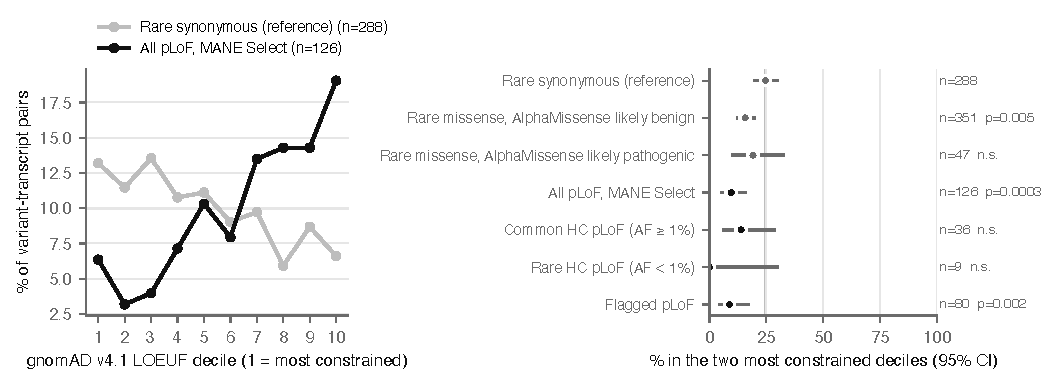
\includegraphics[width=\textwidth]{figures/figS_loeuf.pdf}
\caption{Variant classes of HG002 across gnomAD v4.1 LOEUF deciles. Left:
distribution of all MANE Select pLoF variants and of rare synonymous
variants. Right: share in the two most constrained deciles with 95\%
Wilson intervals; $p$-values from Fisher's exact test against rare
synonymous variants. Units are variant--transcript pairs in MANE Select
transcripts with a LOEUF value.}
\label{fig:loeuf}
\end{figure}

\begin{table}[ht]
\centering\small
\begin{tabular}{lrrrrr}
\toprule
Variant class & $n$ & Deciles 1--2 (\%) & Odds ratio & $p$ & Median LOEUF \\
\midrule
Rare synonymous (reference) & \LoeufSynN & \LoeufSynPct & -- & -- & \LoeufSynMedian \\
Rare missense, AM likely benign & \LoeufAmLbN & \LoeufAmLbPct & \LoeufAmLbOr & $\LoeufAmLbP$ & \LoeufAmLbMedian \\
Rare missense, AM likely pathogenic & \LoeufAmLpN & \LoeufAmLpPct & \LoeufAmLpOr & $\LoeufAmLpP$ & \LoeufAmLpMedian \\
All pLoF, MANE Select & \LoeufAllPlofN & \LoeufAllPlofPct & \LoeufAllPlofOr & $\LoeufAllPlofP$ & \LoeufAllPlofMedian \\
High-confidence pLoF, AF $\geq$ 1\% & \LoeufHcCommonN & \LoeufHcCommonPct & \LoeufHcCommonOr & $\LoeufHcCommonP$ & \LoeufHcCommonMedian \\
High-confidence pLoF, AF $<$ 1\% & \LoeufHcRareN & \LoeufHcRarePct & \LoeufHcRareOr & $\LoeufHcRareP$ & \LoeufHcRareMedian \\
Flagged pLoF & \LoeufFlaggedN & \LoeufFlaggedPct & \LoeufFlaggedOr & $\LoeufFlaggedP$ & \LoeufFlaggedMedian \\
\bottomrule
\end{tabular}
\caption{Share of each variant class in the two most LoF-intolerant LOEUF
deciles. AM, AlphaMissense; odds ratios and Fisher's exact test against rare
synonymous variants.}
\label{tab:loeuf}
\end{table}

\subsection{Clinically classified variants and their parental origin}
A single HG002 variant has a pathogenic or likely pathogenic ClinVar
classification with at least one review star:
\textit{\PlpGene} \PlpHgvsp{} (Table~\ref{tab:rarelof}), the factor~XI
``type~II'' allele (Glu117Ter in the legacy numbering of the mature
protein), heterozygous and inherited from the \PlpParent{}. Its gnomAD
frequency is \PlpAf\% overall but \PlpAsj\% in the Ashkenazi Jewish samples,
\PlpFold-fold higher, consistent with its known founder origin and with the
ancestry of the trio. Founder effects affect the rare pLoF variants more
generally: \NRareAsjCommon{} of the \NHcRare{} variants that are rare in
gnomAD overall have a frequency of at least 1\% in the Ashkenazi Jewish
samples. ClinGen curates \textit{F11} as semidominant; the variant would
therefore be reported as a carrier finding with possible partial factor~XI
deficiency, which this analysis does not assess.

Streaming the parental benchmark VCFs from S3 and the parental benchmark
regions over HTTPS resolves the origin of 9 of the 10 rare high-confidence
pLoF variants (\NRareMaternal{} maternal, \NRarePaternal{} paternal, one
homozygous variant carried by both parents); none is a candidate
\emph{de novo} variant. The unresolved variant, a 168-bp deletion in
\textit{HLA-DQB1}, lies outside the parental benchmark regions. The
homozygous variant illustrates a limit of transcript-level LoF calling: a
45-bp deletion that removes the canonical exon~2 splice donor of the MANE
Select transcript of \textit{PEX5}, whose biallelic loss of function causes
Zellweger spectrum disorder. The same exon has an alternative donor 45\,bp
downstream, and transcripts using it are annotated with an in-frame deletion.
Both parents are homozygous for the deletion, which is absent from gnomAD
and has conflicting classifications in ClinVar; the absence from gnomAD
reflects the length of the deletion rather than its rarity, and the variant
is most probably not a loss of function.

\begin{table}[ht]
\centering\scriptsize\setlength{\tabcolsep}{3pt}
\begin{tabular}{llp{0.2\textwidth}lllllll}
\toprule
Gene & Position & HGVS & Consequence & GT & AF & ASJ AF & ClinVar & MOI & Origin \\
\midrule
\tabinput{results/tex/tab_hc_rare.tex}
\bottomrule
\end{tabular}
\caption{Rare (gnomAD AF $<$ 1\%) high-confidence pLoF variants of HG002.
AF: maximum of the gnomAD exome and genome frequencies; ASJ AF: Ashkenazi
Jewish samples; MOI: ClinGen mode of inheritance (Moderate or stronger
gene--disease validity; SD, semidominant); origin from the parental
benchmark VCFs.}
\label{tab:rarelof}
\end{table}

\subsection{Callability of clinically relevant genes}
A negative result is informative only where the genome has been assessed.
\texttt{coverage()} of the MANE Select coding sequence by the HG002
benchmark regions shows that \NManeGenesLtNinety{} of \NManeGenes{} genes
and \NClinGenLtNinety{} of the \NClinGenGenes{} genes with a ClinGen
gene--disease relationship of at least moderate strength have less than 90\%
of their coding sequence in the benchmark (\NClinGenLtFifty{} less than 50\%;
Figure~\ref{fig:callability}, Table~\ref{tab:callability}). For
\NClinGenLtNinetyDifficult{} of these genes, most of the coding sequence lies
in GIAB difficult regions, such as segmental duplications, tandem repeats
or extreme GC content. \ClinGenFalseDup{} overlap regions that are falsely
duplicated in GRCh38; \textit{CBS}, the gene of classic homocystinuria, has
39\% of its coding sequence in the benchmark.

\begin{figure}[ht]
\centering
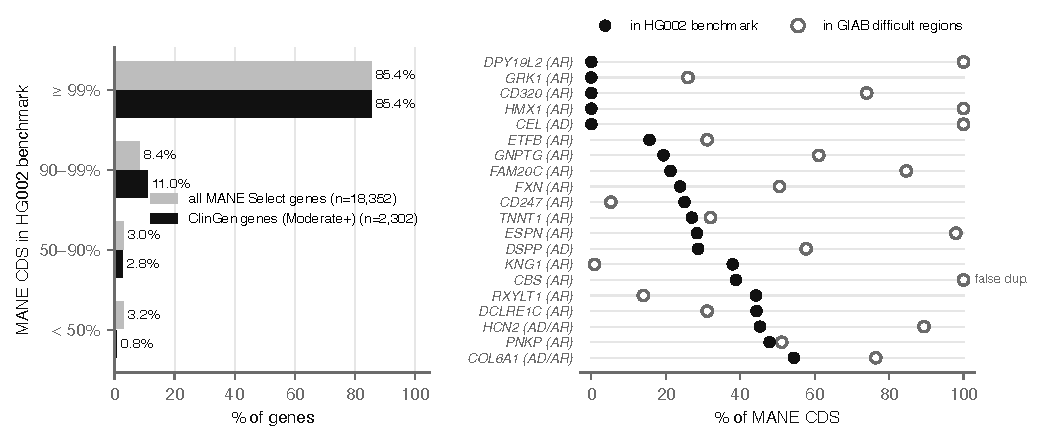
\includegraphics[width=\textwidth]{figures/figS_callability.pdf}
\caption{Share of the MANE Select coding sequence within the HG002 v4.2.1
benchmark regions. Left: genes binned by that share. Right: the 20 least
callable ClinGen genes, with the share of their coding sequence in GIAB
difficult regions (union of all v3.6 stratifications).}
\label{fig:callability}
\end{figure}

\begin{table}[ht]
\centering\scriptsize\setlength{\tabcolsep}{4pt}
\begin{tabular}{lrrrrll}
\toprule
Gene & CDS (bp) & Benchmark (\%) & Segdup (\%) & Difficult (\%) & MOI & Disease (ClinGen) \\
\midrule
\tabinput{results/tex/tab_callability.tex}
\bottomrule
\end{tabular}
\caption{The 25 ClinGen genes with the smallest share of MANE Select coding
sequence in the HG002 benchmark regions.}
\label{tab:callability}
\end{table}

\FloatBarrier
\subsection{Run time}
Annotation of the \NVariants{} variants with the core cache and four plugin
caches took \AnnotateSec\,s with \Workers{} workers; the remaining analysis,
including reading the \NRemoteSources{} ad hoc sources (\RemoteRows{}
million records in total) from their URLs in \RemoteSec\,s, took
\AnalyzeMin\,min, in a single Python process without intermediate VCF, BED
or index files. The tier-3 sources were not converted into caches: a change
of the question (another gene set, another stratification, another relative)
changes only the URL.

\subsection{Conclusions}
The example uses each tier for what it does best. The core cache supplies
VEP-identical consequences and population frequencies for 4.1 million
variants in minutes; plugin caches add frequently updated or licensed
evidence without rebuilding the core; and ad hoc sources answer
analysis-specific questions---gene constraint, curated disease genes, gene
models, genome stratifications and parental genotypes---through joins and
interval operations on the annotated frame. Biologically, the single genome
reproduces the depletion of LoF variants from constrained genes, recovers
the Ashkenazi founder allele \textit{F11} \PlpHgvsp{} with its parental
origin, and identifies the clinically relevant genes in which a negative
result would not be informative.
